%%%%%%%%%%%%%%%%%%%%%%%%%%%%%%%%%%%%%%%%%%%%%%%%%%%%%%%%%%%%
\section*{Introduction and state of the art}
%\subsection{Neutrinoless double beta decay.}
Neutrinos, unlike the other fermions of the Standard Model of particle physics, could be Majorana particles, that is, indistinguishable from their antiparticles. The existence of Majorana neutrinos would have profound implications in particle physics and cosmology. In particular 
the discovery of Majorana neutrinos could be linked to the origin of the matter-antimatter asymmetry observed in the Universe today. 

The only practical way to establish experimentally whether neutrinos are their own antiparticles, and whether lepton number is not conserved, is the detection of neutrinoless double beta decay (\bbonu). This is a hypothetical, very slow nuclear transition in which a nucleus with $Z$ protons decays into a nucleus with $Z+2$ protons and the same mass number $A$, emitting two electrons that carry essentially all the energy released (\Qbb). The process can occur if and only if neutrinos are Majorana particles. 

%%%%%%%%%%%%%%%%%%%%%%%%%%%%%%%%%%%%%%%%%%%%%%%%%%%%%%%%%%%%
\subsection*{The experimental landscape}
The detectors used in double beta decay searches are designed to measure the energy of the radiation emitted by a \bb\ source. In the case of \bbonu, the sum of the kinetic energies of the two released electrons is fixed by the mass difference between the parent and the daughter nuclei: $Q_{\bb} \equiv M(Z,A)-M(Z+2,A)$. However, due to the finite energy resolution of any detector, \bbonu\ events are reconstructed within an energy region centered around \Qbb, typically following a gaussian distribution (Region of Interest, or ROI). Other processes occurring in the detector can fall in the ROI, becoming a background and compromising drastically the expected sensitivity. It follows that \bbonu\ experiments require {\bf excellent energy resolution}, and indeed the field has been traditionally dominated by germanium calorimeters, devices with superb resolution. However, {\bf additional experimental signatures} that allow the distinction between signal and background are needed when the detector exposure (target mass $\times$ time) increases. 
 
 \subsection*{Recent results}
 Three new-generation experiments, with fiducial masses in the range of 100~kg, have recently published the results of their searches for \bbonu\ processes. These are: GERDA, a high resolution calorimeter based on \GE\ diodes; KamLAND-Zen, a low resolution, high-mass, self-shielding liquid scintillator calorimeter, with xenon dissolved in the scintillator; and EXO-200, a liquid xenon (LXe) TPC. All the experiments published null results and therefore a lower limit on the period of \bbonu\ processes, \Tonu. This lower limit can be translated into an upper limit on the \emph{effective Majorana mass} of the electron neutrino defined as:
\begin{equation}
\mbb = \Big| \sum_{i} U^{2}_{ei} \ m_{i} \Big| \, ,
\end{equation}
%
where $m_{i}$ are the neutrino mass eigenstates and $U_{ei}$ are elements of the neutrino mixing matrix. The mass \mbb\ is related to the period through the equation:

\begin{equation}
(T^{0\nu}_{1/2})^{-1} = G^{0\nu} \ \big|M^{0\nu}\big|^{2} \ \mbb^{2} \, .
\label{eq:Tonu}
\end{equation}

In Eq.~\ref{eq:Tonu}, $G^{0\nu}$ is an exactly-calculable phase-space integral for the emission of two electrons and $M^{0\nu}$ is the nuclear matrix element (NME) of the transition, which has to be evaluated theoretically. The uncertainty in the NME affects the value of \mbb\ which can be obtained from \Tonu.
 
{\bf GERDA} \footcite{Agostini:2013mzu} has a resolution of $\sim$0.2 \% FWHM around the \Qbb\ of \GE. This corresponds to a ROI of about 4 keV. The specific background rate in the ROI is $10^{-2}$ \ckky, and therefore the number of background counts in the ROI is 0.4 per kilogram or 40 per ton. The total exposure deployed is 21.6 kg$\cdot$yr. The experiment sets a limit $\Tonu(\GE)> 2 \times 10^{25}$~yr, which translates into an upper limit range for \mbb\ of $[258-649]$~milli electronvolts (meV). The bracket reflects the uncertainty in the NME.

{\bf EXO} \footcite{Albert:2014awa} achieves an energy resolution of 3.6\% FWHM at \Qbb, and a background rate of $ 4 \times 10^{-3}\ckky$ (thus about 35 events per ton in the ROI). The total exposure used for the published result is 100 kg$\cdot$~yr. The EXO Collaboration has published a limit on the half-life of \bbonu\ in \XE\ of $T_{1/2}^{0\nu}(\XE) > 2 \times 10^{25}$~yr. The limit translates into an upper limit range for \mbb\ of $[125-352]$~meV, depending on the NME.

{\bf KamLAND-Zen} \footcite{TheKamLAND-Zen:2014lma} compensates a worse energy resolution of 10\% FWHM at \Qbb\ with a very small background rate of $\sim 8 \times 10^{-4}$ \ckky (20 events per ton in the ROI). After an exposure of 108.8 kg$\cdot$~yr, they obtain a limit  $T_{1/2}^{0\nu}(\XE) > 2.6 \times 10^{25}$~yr, which translates into an upper limit range for \mbb\ of $[110-309]$~meV, depending on the NME.

 \subsection*{Potential for discovery}
 
% %%%%%%
%\begin{figure}
%\centering
%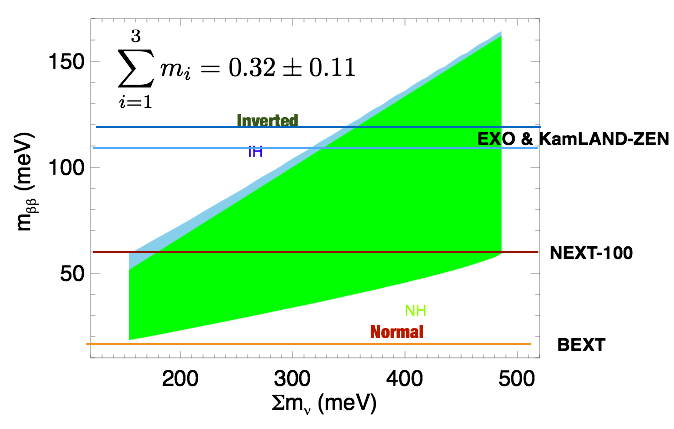
\includegraphics[width=0.70\textwidth]{img/SensiCRR.png}
%\caption{\small The allowed \mbb\ region (68\% CL for two degrees of freedom), as a function of the sum of the neutrino masses, assuming that 
%$\sum m_i = 0.32\pm 0.11$~eV. The blue lines mark the sensitivity of EXO and KamLAND-ZEN, the xenon-based detectors currently leading the field. The red line shows the sensitivity of NEXT after 3 years operation.} 
%\label{fig.mbb}
%\end{figure}
%%%%%%

 Several analyses from recent cosmological results suggest that the sum of the masses of the three neutrinos could be $\sim$ 0.3 eV\footcite{PhysRevLett.112.051303}. G\'omez-Cadenas and collaborators have demonstrated that, in this case, if the neutrino is a Majorana particle, then, $\mbb \sim [20-150]$~ meV \footcite{GomezCadenas:2013ue}. Therefore, experiments capable of exploring the ``cosmologically relevant region'' (CRR, corresponding to \mbb\ between  20 and 150 meV), would have a chance of making a discovery.
 
 %as shown in Figure \ref{fig.mbb}. 
It is sobering to notice that  the sensitivity of GERDA (\mbb\ $\sim$ [258-649]) is outside the CRR, while both EXO-200 (\mbb\ $ \sim [125-352]$) and KamLAND-Zen ( \mbb\ $ \sim [110-309]$) would have already explored a significant fraction of CRR {\em only for the most optimistic NME set} (while they would be outside CRR for the most pessimistic). 
 Clearly, the experimental effort to determine if the neutrino is a Majorana particle, is far from being completed is, rather, in its infancy. 
 %To establish unambiguously that the neutrino is (or not) a Majorana particle, even in this favourable scenario in which the sum of the neutrino masses is relatively high, experiments must be sensitive to $\mbb \sim 20$~meV, {\em even for the most pessimistic NME} set. This is a major challenge.
% 
 
%%%%%%%%%%%%%%%%%%%%%%%%%%%%%%%%%%%%%%%%%%%%%%%%%%%%%%%%%%%%
\section*{The NEXT experiment and its innovative concepts}
\begin{figure}
\centering
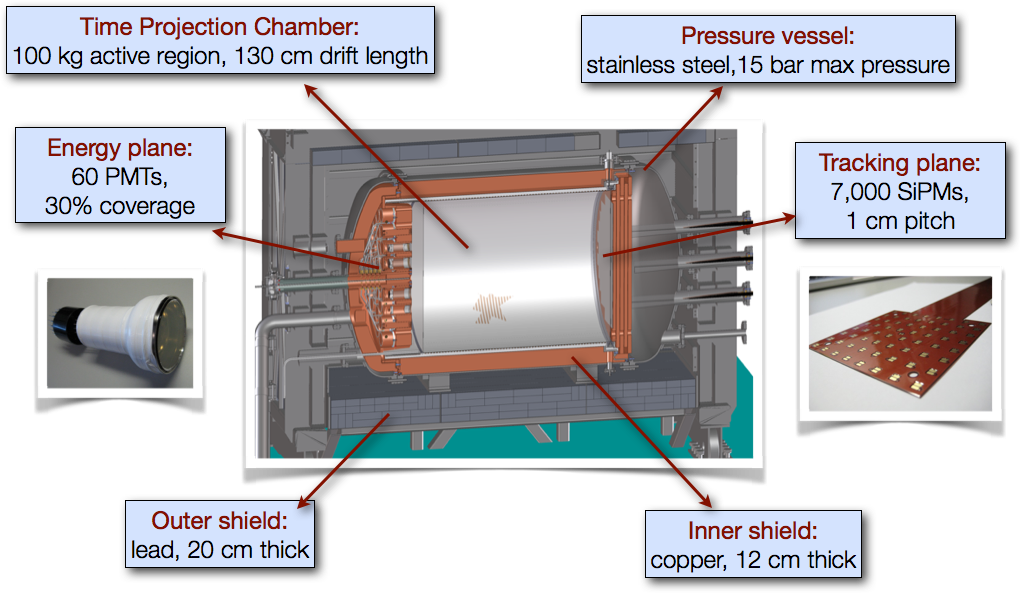
\includegraphics[width=0.9\textwidth]{img/NEXT.png}
\caption{\small A drawing of the NEXT-100 detector showing its main parts. The pressure vessel (PV) is made of a radio pure steel-titanium alloy. The PV dimensions are 130~cm inner diameter, 222~cm length, 1~cm thick walls, fot a total mass of 1\,200 kg. The inner copper shield (ICS) is made of ultra-pure copper bars and is 12~cm thick, with a total mass of 9\,000 kg. The time projection chamber includes the field cage, cathode, EL grids and HV penetrators.
The light tube is made of thin teflon sheets coated with TPB (a wavelength shifter). 
The energy plane is made of 60 PMTs housed in copper enclosures (cans).
The tracking plane is made of MPPCs arranged into dice boards (DB). 
} \label{fig.NEXT100}
\end{figure}

The \emph{Neutrino Experiment with a Xenon TPC} (NEXT)\footcite{next} will search for \bbonu\ in \XE\ using  high-pressure xenon gas  time projection chambers (\HPXE). The advantages of the technology are: 
a) {\bf excellent energy resolution}, with an intrinsic limit of about 0.3\% FWHM at \Qbb, close to that of \GE\ detectors, and a proved performance of 0.5 \% FWHM; b)
{\bf tracking capabilities} that provide a powerful topological signature to discriminate between signal (two electron tracks with a common vertex) and background (mostly, single electrons); c)
{\bf a fully active and homogeneous detector}, with no dead regions; d) {\bf scalability} of the technique to large masses. 

The design of the NEXT-100 detector (Figure \ref{fig.NEXT100}) is optimised for energy resolution by using proportional electroluminescent (EL) amplification of the ionisation signal. The detection process involves the use of the prompt scintillation light from the gas as start-of-event time, and the drift of the ionisation charge to the anode by means of an electric field ($\sim0.3$ kV/cm at 15 bar) where secondary EL scintillation is produced in the region defined by two highly transparent meshes, between which there is a field of $\sim20$ kV/cm at 15 bar. The detection of EL light provides an energy measurement using photomultipliers (PMTs) located behind the cathode (the \emph{energy plane}) as well as tracking through its detection a few mm away from production at the anode, via a dense array of silicon photomultipliers (the \emph{tracking plane}).

\subsection*{The NEXT-DEMO prototype}

\begin{figure}
\centering
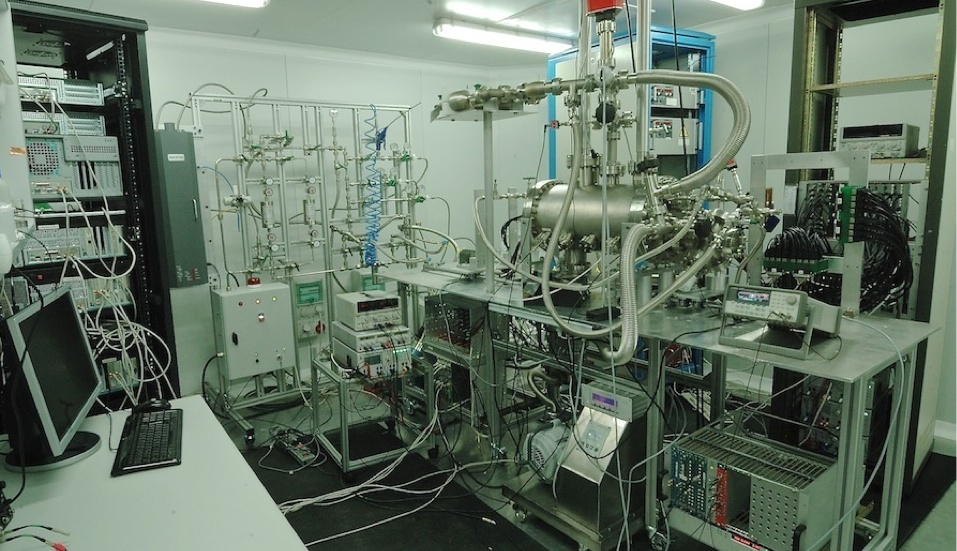
\includegraphics[width=0.9\textwidth]{img/DemoSetup.jpg}
\caption{\small The NEXT-DEMO prototype setup. 
%Top-left: the pressure vessel, showing the HVFT and the mass spectrometer; bottom-left: an expanded view of the detector; (c) Teflon light tube; (d) energy plane, made of pressure resistant Hamamatsu R7378A PMTs; (e) field cage; (f) tracking plane equipped with 300 Hamamatsu MPPCs; top-right: the full setup at IFIC; bottom right: the field cage.
} \label{fig.DEMO}
\end{figure}
%%%%%%%%%%

%\begin{figure}
%\centering
%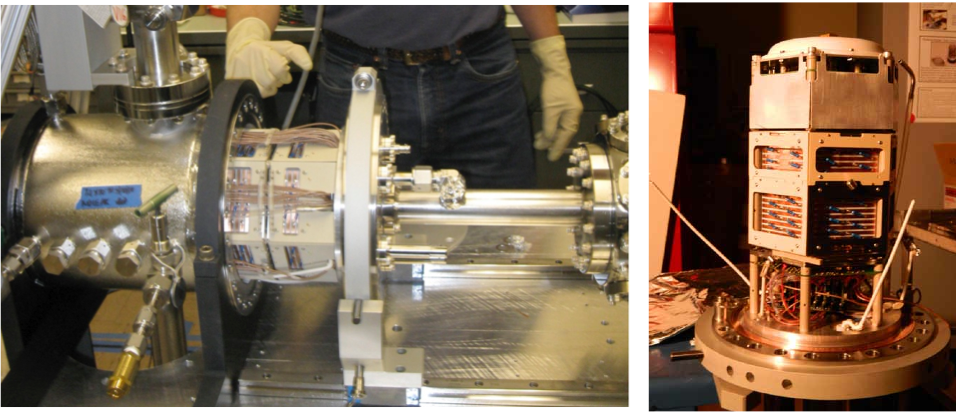
\includegraphics[width=0.99\textwidth]{img/DBDM.png}
%\caption{\small The NEXT-DBDM prototype. Top-left: the pressure vessel, in the moment in which the field cage is inserted; (b) the field cage.} \label{fig.DBDM}
%\end{figure}


NEXT-DEMO, shown in figure \ref{fig.DEMO}, is as a large-scale prototype of NEXT-100. The pressure vessel has a length of 60 cm and a diameter of 30 cm. The vessel can withstand a pressure of up to 15 bar and hosts typically 1-2 kg of xenon. NEXT-DEMO is  equipped with an energy plane made of 19 Hamamatsu R7378A PMTs and a tracking plane made of 256 Hamamatsu SiPMs. 

The detector has been operating successfully at IFIC since 2011 and has demonstrated: (a) very good stability, with no leaks and very few sparks; (b) good energy resolution ; (c) track reconstruction with PMTs and with SiPMs coated with TPB; (d) excellent electron drift lifetime, of the order of 20 ms.Its construction, commissioning and operation has been instrumental in the development of the required knowledge to design and build the NEXT detector.

%The NEXT-DBDM prototype (Figure \ref{fig.DBDM}) is a smaller chamber, with only 8 cm drift, but an aspect ratio (ratio diameter to length) similar to that of NEXT-100. The device has been used to perform detailed energy resolution studies, as well as studies to characterise neutrons in an \HPXE. NEXT-DBDM achieves a resolution of 1\% FWHM at 660 keV and 15 bar, which extrapolates to 0.5\% at \Qbb.

%\subsection*{Topological signature and energy resolution}
%
%%%%%%
%\begin{figure}
%\centering
%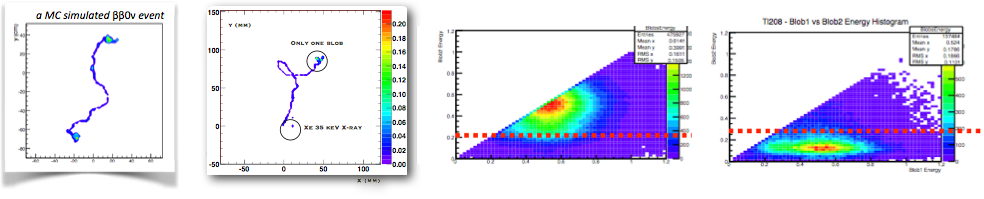
\includegraphics[width=0.99\textwidth]{img/TOPO.png}
%\caption{\small NEXT has a topological signature, not available in most \bbonu\ detectors. The panel shows the reconstruction of a Monte Carlo signal (topleft) and background (second from left) event. The signal has two electrons (two blobs). The background has only one electron (one blob) and the associated emission of a 35 keV X-ray. The color codes energy deposition in the TPC. An scatter plot of the energy of the two blobs shows a clear separation between signal and background regions.}\label{fig.ETRK2}
%\end{figure}
%%%%%

%%%%%%
%\begin{figure}
%\centering
%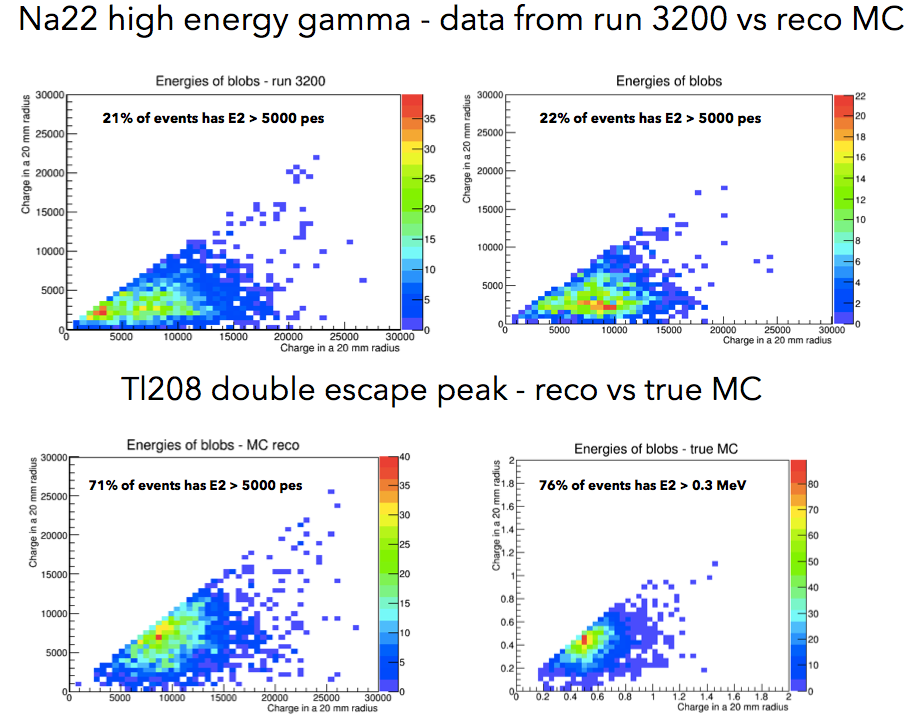
\includegraphics[width=0.9\textwidth]{img/ElectronsDataMC.png}
%\caption{\small A comparison between data (left) and Monte Carlo (right) for electrons of different energies recorded in the DEMO chambers, showing the very good agreement between both data sets and therefore the robustness of the topological signal, unique of the NEXT experiment.}\label{fig.ETRK3}
%\end{figure}


%Double beta decay events leave a distinctive topological signature in HPXe: a continuous track with larger energy depositions (\emph{blobs}) at both ends due to the Bragg-like peaks in the d$E$/d$x$ of the stopping electrons (figure \ref{fig.ETRK2}, topleft). In contrast, background electrons are produced by Compton or photoelectric interactions, and are characterised by a single blob and, often, by a satellite cluster corresponding to the emission of $\sim30$-keV fluorescence x-rays by xenon (figure \ref{fig.ETRK2}, bottomleft).
%Reconstruction of this topology using the tracking plane provides a powerful means of background rejection, as can be observed in the figure. In our TDR we chose a conservative cut to separate double--blob from single--blob events which provided a suppression factor of 20 for the background while keeping 80\% of the signal.  DEMO has reconstructed single electrons from \NA\ and \CS\ sources, as well as double electrons from the double escape peak of \TL\, demonstrating the robustness of the topological signal. 

%
%Figure \ref{fig.ETRK3} shows a comparison between data and Monte Carlo for electrons interacting in the DEMO detector. Two radioactive sources were used: Na-22, producing single electrons of 511 keV, and Tl-208, whose double escape peak produced {\em double electrons}, at the energy of 1.6 MeV. Both data sets allow us to ``mimic'' signal and background and thus have a robust assessment of the performance of the topological signal comparing the Monte Carlo simulation and the actual results obtained with DEMO. The agreement between both data sets is very good, revealing the robustness of the topological signal. 

%\subsection{Energy resolution}

%%%%%
%\begin{figure}
%\centering
%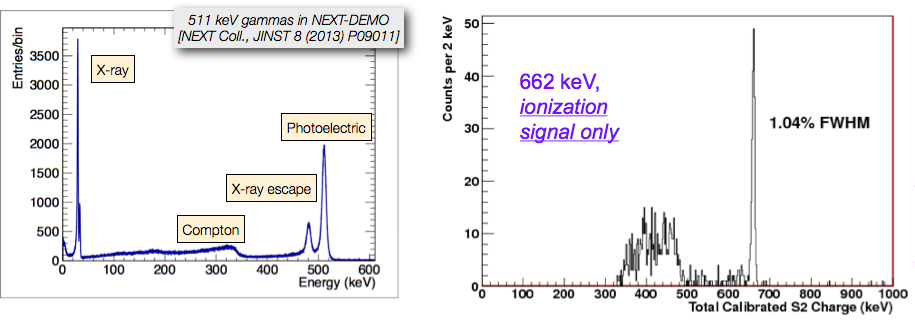
\includegraphics[width=0.9\textwidth]{img/EResolution.png}
%\caption{\small Left: the full energy spectrum measured for electrons of 511 keV in the DEMO detector. Right the spectrum near the photoelectric peak for 662 keV. The extrapolated resolution is 0.7\%.}\label{fig.ERES}. 
%\end{figure}
%%%%%
%
%Figure \ref{fig.ERES} shows the resolution obtained with NEXT-DEMO, which extrapolates to 0.7\% FWHM at \Qbb.
%
The status of the NEXT experiment and the results achieved by the prototypes have been described in a recent
paper \footcite{Gomez-Cadenas:2013lta}. The first phase of the detector is currently being installed at the Canfranc underground laboratory (LSC). 


%\subsection{\label{sec.new}The NEW detector.}
%
%%%%%%%%%%%
%\begin{figure}
%\centering
%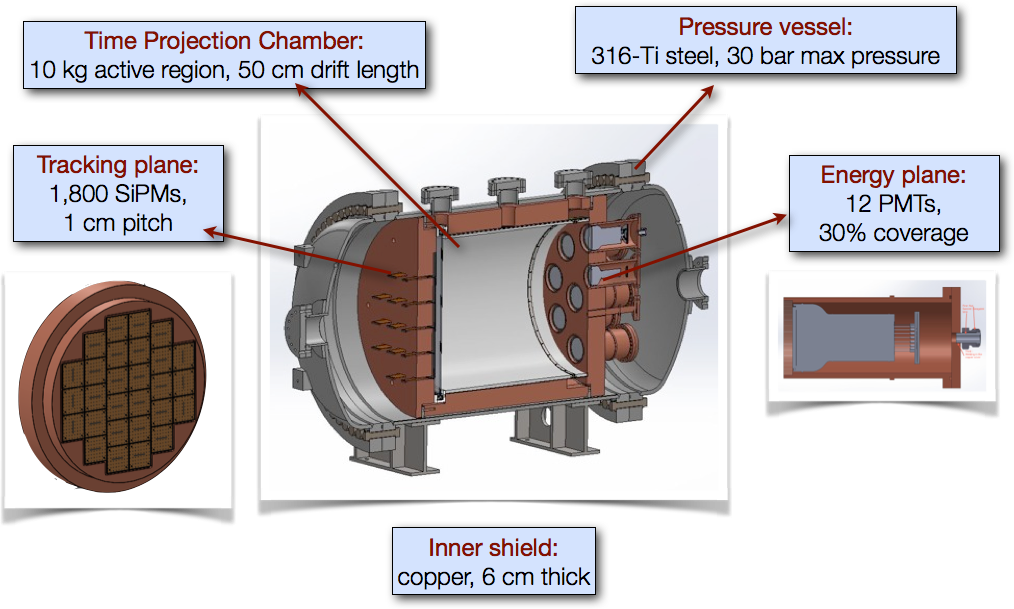
\includegraphics[height=9cm]{img/NEW.png}
%\caption{\small The NEW apparatus.} \label{fig:NEW}
%\end{figure} 
%
%The NEW (NEXT-WHITE) apparatus\footnote{The name honours the memory of the late Professor James White, one of the key scientists of the NEXT Collaboration.}, shown in Figure \ref{fig:NEW}, is the first phase of the NEXT detector to operate underground. NEW 
%%has a triple goal:
%
%\begin{enumerate}
%\item {\bf Technology}: it will validate the technological solutions adopted by NEXT-100.
%\item {\bf Radiopurity}: it will allow the NEXT collaboration an extra step in the implementation of a radiopure detector.
%\item {\bf Physics}: it will demonstrate with measurements of the \BI\ and \TL\ lines, as well as with the measurement of the \bbtnu\ spectrum, the physics capabilities of NEXT-100.
%\end{enumerate}
%
%is a scale 1:2 in size (1:8 in mass) of NEXT-100. The energy plane contains 12 PMTs (20 \% of the 60 PMTs deployed in NEXT-100). The tracking plane technology consists of 30 Kapton Dice Boards (KDB) deploying 1800 SiPMs (also 20\% of the sensors). The field cage has a diameter of 50~cm and a length of 60~cm (the dimensions of the NEXT-100 field cage are roughly 1~m long and 1.2~m diameter). 
%
%NEW is a necessary step\footnote{As formally stated by the scientific committee of the LSC, who recommended its construction in 2013.} towards the construction of NEXT-100. It will validate the technological solutions adopted by the collaboration and, as discussed below, it is essential in the definition of the project methodology. Furthermore, The NEXT background model is currently based on a sophisticated Monte Carlo simulation of all expected background sources in each part of the detector. NEW will allow the validation of the background model with actual data. 
%%Last but not least, NEW operation will demonstrate with measurements of the \BI\ and \TL\ lines, as well as with the measurement of the \bbtnu\ spectrum, the physics capabilities of NEXT-100.
%
%Furthermore, the calibration of NEW with 
%sources of higher energy, will allow a precise study of the evolution of the resolution with the energy. 
%In particular it will be plausible to measure the resolution near \Qbb\ using a Thorium source, which provides 2.6 MeV gammas. Last, but not least, we intend to 
%reconstruct the spectrum of \bbtnu. Those events are topologically identical to signal events (\bbonu) and can be used to demonstrate with data the power of the topological signature. 
%%

\subsection*{Discovery potential of NEXT-100.}

The excellent resolution of NEXT (0.7 \% FWHM), and the combination of a low radioactive budget with a topological signature, which yields an expected background rate of $5 \times 10^{-4} \ckky$, (thus less than 10 events per ton) will allow the NEXT-100 detector to reach a sensitivity to the \bbonu\ period of $\Tonu > 7 \times 10^{25}$~yr for a exposure of 300 kg$\cdot$yr. This translates into a \mbb\ sensitivity range as low as $[67-187]$~meV, depending on the NME. Therefore NEXT-100 will have a substantial chance of making a discovery if the NME is sufficiently high. 

\section*{Towards a ton-scale high-pressure xenon TPC.}

%%%%%%%
%\begin{figure}
%\centering
%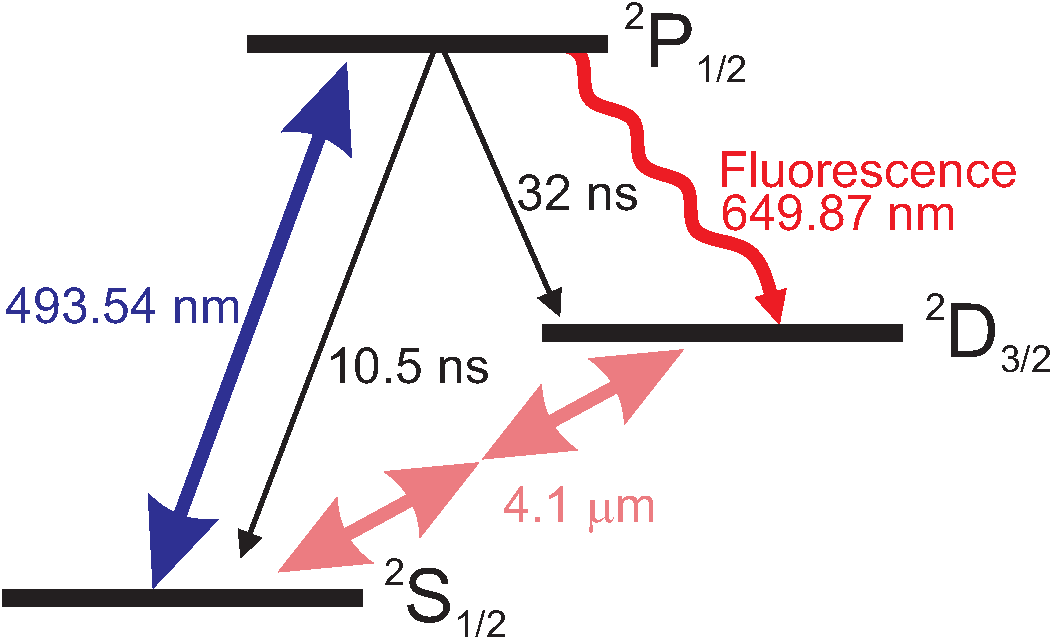
\includegraphics[width=0.60\textwidth]{img/levelscheme2.pdf}
%\caption{\small The \BATA\ concept.} \label{fig.BATA}
%\end{figure}
%%%%%%

If no discovery is made by the current generation of experiments, the full exploration of the CRR region (corresponding to \mbb\ values as low as 20~meV) requires detectors of larger mass (at least 1 ton), good resolution and extremely low specific background. The \HPXE\ technology has the potential to provide the most sensitive detector at this scale, by scaling the detector to a mass in the range of one ton and adding additional handles to further suppress the background. 

%\subsection{Barium Tagging}
%
%One of the most promising possibilities is to develop the technology to unambiguously tag the barium ion produced in the xenon decay, $Xe \rightarrow Ba^{++} + 2 e^-$. The conceptual idea to tag $Ba^{+}$ is illustrated in Figure \ref{fig.BATA}. A ``blue'' laser of wavelength 493.54 nm excites (``pumps'') the S state, inducing $S \rightarrow P$~transitions, with a lifetime of $\sim$ 10 ns. About 30 \% of the times the \TwoP\ states decay to the state \TwoD, emitting ``red'' (649.76 nm) fluorescence in a characteristic time of 30 ns. The state \TwoD\ is metastable, but a second laser of suitable wavelength (4.1 $\mu$m) can be used to induce the transition to the ground state (this is known as ``deshelving'').  The whole cycle takes less than 50 ns, and therefore several millions of red fluorescence photons can be emitted by a single ion. 
%
%The practical application of this conceptual idea is by no means easy, and in fact, it has been shown to be extremely difficult in liquid xenon by the work of the EXO collaboration\footcite{Dolinski:2012dta}. However, it may be feasible in a \HPXE\ detector, where a number of fortunate conditions may occur. These conditions are: a) charge reduction of the emitted barium ion, from $Ba^{++}$~to $Ba^{+}$, which can be induced by collisions with xenon atoms, or by the addition of a suitable quencher; b) ``trapping'' of the barium ion ``in situ'' by the surrounding Xe atoms, which result in a very low drift velocity for the ion; c) location of the ion, via the reconstruction of the event topology. 
%
%All the above needs to be demonstrated with a systematic R\&D program, which must also address additional experimental issues such as pressure broadening of the laser, filtering of Rayleigh scattering, and others. The EXO collaboration has carried out extensive research of the potential for Barium Tagging, not only in a LXe TPC, but also in an \HPXE, where promising results are obtained\footnote{See for example, {\em MOBILITY AND FLUORESCENCE OF BARIUM IONS IN XENON GAS FOR THE EXO EXPERIMENT},
%Ph.D. thesis, Julio Cesar Benitez Medina, Department of Physics
%Colorado State University,
%Spring 2014.}. NEXT, on the other hand, has started a collaboration with CLPU\footcite{clpu}, a Spanish national facility dedicated to ultra-intense lasers, with the aim of carrying out a systematic R\&D program to understand the potential of Barium Tagging in a high pressure gas xenon TPC. We believe that such a program offers also a unique opportunity of joint development with the EXO collaboration. Clearly the construction of a ton-scale \HPXE\ detector implementing the full Barium Tagging technology is a very challenging enterprise. On the other hand, it appears to be a promising path towards the future. 
%

\subsection*{Adding a magnetic field to enhance the topological signal}

%%%%%%%
\begin{figure}
\centering
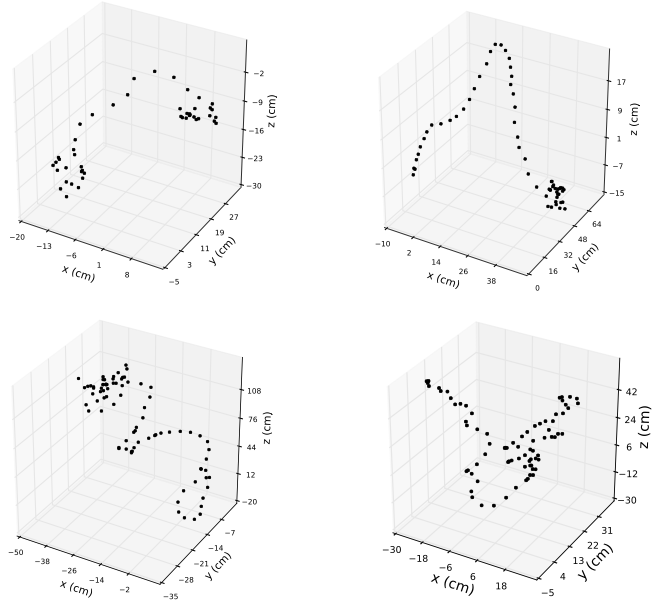
\includegraphics[width=0.7\textwidth]{img/TRACKS2.png}
\caption{\small Top Left: two electrons emitted in a \bbonu\ decay in the absence of magnetic field. Top right: a single (background) electron produced by the photoelectric interaction of a 2.45 MeV photon emitted in \BI\ decays, interacting in the chamber. Bottom left: two  electrons emitted in a \bbonu\ decay, turning into a double helix that originate in a common vertex, in a magnetic field of 0.5 T. Bottom right: a single background electron turning into a single helix in a magnetic field of 0.5 T. } \label{fig.KF}
\end{figure}
%%%%%%

The simplest way to improve the \HPXE\ technology is to operate the detector in a moderate magnetic field. 
In the presence of a uniform external magnetic field $B$, charged particles spiral around the field lines in circular motion with radius $r = p_T/eB$, where $p_T$~ is the momentum of the electron transverse to the direction of the field and $e$~ is the electron charge. A single energetic electron should produce a clear single spiral with radius indicative of its momentum, and a double-electron track with the same energy will produce two spirals each with much less momentum and originating from a common vertex. This information provides an additional way of separating single-electrons arising from background processes from double electrons produced in \bbonu\ decays, {\bf in spite of the large multiple scattering that the electrons suffer in a dense \HPXE}. 

This is illustrated in Figure \ref{fig.KF}. The top-left panel shows two electrons emitted in a \bbonu\ decay in the absence of magnetic field. Notice that the vertex where both electrons originated cannot be easily measured due to multiple scattering. However, the presence of two electrons is revealed by the two blobs at the end of the tracks (regions with higher density of hits and energy deposition, which originate when each one of the electron ranges out). Instead, the top-right panel shows a single background electron, which originates inside the detector when a photon, emitted by the decay of the isotope \BI\ enters the chamber and suffers a photoelectric interaction. (\BI\ appears in the natural uranium chain, and is present in small trace activities in the detector materials). Notice that the single electron only displays one blob in one of the vertexes. Thus, even in the absence of magnetic field, single and double electrons can be separated. 

However, when a sufficiently intense magnetic field is added, the separation between single and double electrons is strongly enhanced. The bottom-left panel shows again two electrons emitted in a \bbonu\ decay, turning in a magnetic field of 0.5 Tesla. The trajectory shows clearly two helices, originating from a common vertex, which becomes now visible. The bottom-right panel shows a single background electron turning in a 0.5 T magnetic field, following a single helix. Fitting the trajectories of the electrons, one can achieve an additional order of magnitude in background reduction with respect to the case without magnetic field, combining the fact that the signal is now characterised by two blobs and two helices pointing towards a common vertex.    

%Multiple scattering occurs as an energetic electron traverses a dense medium --it undergoes several large-angle scatters that sharply divert an otherwise relatively smooth path through the detector, and the variance on angle of these scatters becomes larger at lower momentum--. On the other hand, using the mathematical technique known as the Kalman Filter\footcite{Cervera:2002} and incorporating multiple scattering as a noise process, fits to reconstructed electron tracks in both directions, {\bf assuming they are single-electron tracks with initial momentum corresponding to the kinetic energy released in $\bbonu$},  give different results for single and double-electron tracks, as illustrated in Figure \ref{fig.KF}. For single-electron tracks, the fit should perform well in one direction (from the production vertex to the end vertex, since in this case the fit hypothesis is correct) and poorly in the other direction (from end vertex to production vertex, since now the hypothesis is totally wrong, and the electron has, as the start of the fit, vanishing momentum). For double-electron tracks, the fit should fail in both directions. 
%
%The illustrative result displayed in Figure \ref{fig.KF}\footnote{J.J. Gomez-Cadenas, J. Renner, A. Cervera, J.A. Hernando, A. Imzaylov, F. Monrabal and J. Muñoz, ``Enhancing the topological signature of an HPXe detector by means of a magnetic field'', in preparation.} shows how the ``forward fit'' (from production to end vertex), differs from the ``reverse fit'' (from end vertex to production vertex'').  The right panel of the figure displays the local $\chi^2$~at each step of the fit. In the case of the forward fit (correct hypothesis), the fit converges rapidly to a flat value, since the Kalman Filter keeps updating the momentum o the electron as it losses energy by ionisation. Since the Kalman Filter model incorporates multiple scattering, the trajectory of the electron can indeed be tracked, as shown in the left panel of the figure. Instead, the local $\chi^2$~for the reverse fit is too high at the beginning of the fit (the hypothesis is that the momentum is large, when in fact is is very small, therefore the predicted multiple scattering error is underestimated) and too small at the end of the fit (where the situation is reversed and thus the predicted multiple scattering error is overestimated).  
%
%In the simulation, the assumed point-error is 1 mm. Such a resolution is difficult to achieve in NEXT-100, due to the transverse diffusion of the ionisation electrons as they drift to the anode. However, when a solenoidal magnetic field is added the E$\times$B effect reduces the lateral diffusion to negligible levels for any reasonable value of the field ($B=0.1$~Tesla is used for the simulations). In NEXT-100, position is reconstructed using SiPMs spaced at a pitch of 10 mm, yielding a resolution (if one would not make use of the SiPM recorded charge to weight the event position) of 3 mm, which improves to $\sim$~1 mm when the position is weighted by the SiPM recorded charge. Therefore, the resolution assumed in the plot is correct in the presence of a magnetic field. 

%To further enhance the topological signature of NEXT (see Figure \ref{fig.ETRK2}), one performs a Kalman Fit to double-electron candidates (that is, those which have passed the selection cut requiring that the energy of the two blobs defining the beginning and end of the track is large). As noted, in true signal events, the momentum in each blob vanishes (each blob corresponds to the end-vertex of one of the two electrons emitted in a \bb\ decay). In background events managing to ``fake'' a blob at the start of the track, the fit will succeed in one direction (when we start from the fake blob, in which case the momentum is 2.3 MeV, corresponding to the kinetic energy of \Qbb), and will fail in the other (when we start from the true blob, where the momentum vanishes). Thus, fitting the candidates surviving the standard topological cut of NEXT, {\em under the hypothesis that they are background electrons}, provide an extra rejection criteria for background. We fit the trajectory of the electron starting from both ends, and accept it only if the fit is consistent, in both cases, with a reverse fit.  This simple approach yields a factor 10 extra rejection (for 90\% signal efficiency), {\em in the absence of a magnetic field}.
%
%Indeed, the rejection in the absence of magnetic field comes from an {\em indirect} measurement of the momentum of the electrons through their multiple scattering
%angle $\theta_0$:
%
%\begin{equation}
%\theta_{0} = \frac{13.6}{\beta c p}\sqrt{\frac{x}{X_0}}+(1 + 0.038 \log{\frac{x}{X_0}})
%\end{equation}
%% 
% where $X_0$ is the radiation length of the dense xenon gas 
% $\sim P \times 8.48 ~g\cdot cm^{-2}$~where $P$~is the pressure of the gas) 
% $\beta c$~is the velocity of the electron and $p$~its momentum. 
% 
% When a magnetic field $B$~ is added the (transverse) momentum of the electrons can be 
% directly measured,  $p_T = r \times B$. The determination of $p_T$ does not need to be accurate (which is fortunate, given the fact that the trajectory of the electrons is smeared by multiple scattering), because one applies the strategy described above. Single (background) electrons will yield a good forward fit (where now the momentum of the electron must be consisted with the track curvature) and a bad reverse fit. Double (signal) electrons will yield reverse fits in two directions. Indeed, for candidate signal (double) electrons is is possible to scan the starting point of the reverse fit in both directions, until a good forward fit is found. This corresponds to the vertex of the double electron. 
% 
% Work is in progress to assess the final rejection factor and efficiency obtained when a magnetic field is added (the range of the magnetic field for pressures between 10-20 bar appears to be $\sim$0.1 Tesla) and both topological signatures (blob and vertex signatures) are combined, but our preliminary studies indicate that adding the vertex signature will provide a factor of 10 extra rejection of backgrounds at little cost (90\%) to the signal efficiency.  
 
 The estimated rejection factor for NEXT-100 is less than 10 background counts per ton and year. The addition of a magnetic field will yield a value of less than one count per ton in the ROI, thus allowing the experiment to operate in the ton regime without being background limited. In consequence NEXT can be upgraded to fully explore the CRR and therefore make a discovery if the neutrino is a Majorana particle. 
  
\section*{Demonstrating operation in a magnetic field}

\subsection*{Replacing PMTs with large-area SiPMs}
%%%%%%%
%\begin{figure}
%\centering
%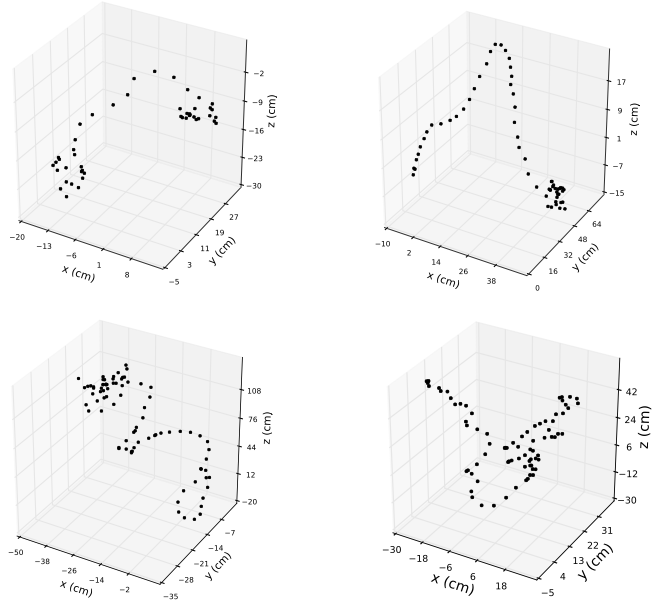
\includegraphics[width=0.9\textwidth]{img/TRACKS2.png}
%\caption{\small Left: gain of the new C-series, SENSL devices (red line) 
%compared with old series. A DC of around ten kHz can be achieved at room
%temperatures for operating voltages around 27-28 Volts. Right: Spread of the breaking voltage, Vbr. The r.m.s. of the distribution is 0.041 V for a mean value of 24.52 (0.16 \% r.m.s.)} \label{fig.SENSL}
%\end{figure}
%%%%%%

The current design of NEXT is based in the use of low-background PMTs for the energy plane. PMTs are excellent sensors for energy measurement, given their capability as single-photoelectron counters. On the other hand, their use limits the potential of the technology. The most important drawback is the fact that PMTs do not work in a magnetic field, but there are other important disadvantages, namely: a) even very radio-pure PMTs contribute significantly to the radioactive budget of the detector; b) there are no available radio-pure PMTs that are also resistant to pressure, and therefore sophisticated engineering is needed to separate a region of vacuum (for PMT operation) from the pressurised volume of the TPC; c) the use of PMTs as energy-measuring devices and SiPMs as tracking devices imposes an asymmetric design to NEXT (with an energy plane behind the cathode and a tracking plane in the anode), while a symmetric design would be preferable (it would allow to increase the detector mass by a factor of two without adding extra sensors, given the very long electron lifetime available in the experiment). 

NEXT has pioneered the use of SiPMs as pixel detectors for the tracking plane, and the DEMO prototype is the first high-pressure xenon TPC in the World to deploy a fully operational tracking plane based in SiPMs. However, until recently, the dark current and high spread in gain (for a fixed operating voltage) of the available SiPMs made them not suitable for energy measurements.

The situation has changed dramatically in the next two years, thanks to the quick evolution of the field. In particular, the NEXT collaboration has been collaborating with the SENSL company\footnote{http://sensl.com/home/} to identify ultra-radio pure SiPMs. We have recently shown\footnote{``Radiopurity assessment of the tracking readout for
the NEXT double beta decay experiment'', the NEXT collaboration, paper submitted to the Seattle IEE conference, November, 2014.} that the C-series, MLP packaging produced by the company is extremely radiopure. In addition, the dark current of the devices can be reduced up to near 10 kHz per mm$^2$, at room temperatures. 
%(Figure \ref{fig.SENSL}, left).  
Last but not least, the spread in operating voltage (therefore in gain) of the devices is very low, of the order of 0.2 \%. 
%((Figure \ref{fig.SENSL}, right shows that the spread in breakdown voltage is around 0.16 \% r.m.s). 
These three break-throughs, together with the affordability of the devices makes it possible to use SiPMs not only as tracking sensors but also to measure the energy of the events, replacing the PMTs. 

\subsection*{Upgrading NEXT-DEMO}
%%%%%%%
\begin{figure}
\centering
\includegraphics[width=0.8\textwidth]{img/DU.png}
\caption{\small Top left: the current tracking plane of NEXT-DEMO is made of 4 dice boards, each one hosting 64 1 mm$^2$ Hamamatsu SiPMs at a pitch of 1 cm. Top right: the current energy plane of DEMO is made of 19 pressure resistant PMTs (non radiopure). Bottom left: the upgraded tracking plane will use the new SENSL C series 1 mm$^2$ SENSL devices mounted in the ultra-low background kapton dice boards (KDBs) developed for NEXT-100.  Bottom right: The upgraded energy plane will use the new SENSL 6$\times$6 mm$^2$~ SiPMs. Each KDB will mount 100 sensors. } \label{fig.DemoUpgrade}
\end{figure}
%%%%%%

Figure \ref{fig.DemoUpgrade} shows the configuration of the DEMO tracking plane and energy plane, and the drawings for the upgrade. For the energy plane, we foresee the use of the largest available SiPMs from the C series, with a size of 6$\times$6 mm$^2$. Each KDB will host 100 SiPMs, connected to a common voltage and the front-end electronics will perform the analog sum of all the devices in a Kapton Dice Board, or KDB (this is possible thanks to the very low spread in gain). For the tracking plane we will deploy 4 of the new KDBs developed for NEXT-100, which will also use C-series SiPMs. 

%An important point: a huge effort and a considerable investment was needed to build, commission and understand the NEXT-DEMO detector. This includes all the hardware and software components that will be re-used for this proposal. Gas system, high voltage and high voltage penetrators, pressure vessel, field cage, front-end electronics, data acquisition, slow controls, online monitoring, reconstruction software, calibration software and Monte Carlo simulation. The upgrade of DEMO, instead, is rather simple for our experienced team. For the tracking plane we can reuse four of the KDBs currently in production for NEXT-100, and the SiPM-energy plane requires a comparatively minor effort in design (the person in charge will be Javier Rodriguez, who is the designer of the NEXT KDBs and the leader of the NEXT electronics group) and production. 

Notice that the cost of the upgrade is a very small fraction of the cost of the whole system, since we will reuse the whole DEMO setup. In addition, the tracking plane will be built with spares KDBs from the production of the NEXT detector, and thus only funding for the energy plane is needed. {\em With this modest investment, the upgraded DEMO detector will be the first system of its kind to measure energy with high resolution using a SiPM based technology.} 

\subsection*{Operating NEXT-DEMO inside the TPC90 Magnet at CERN}
%%%%%%%
\begin{figure}
\centering
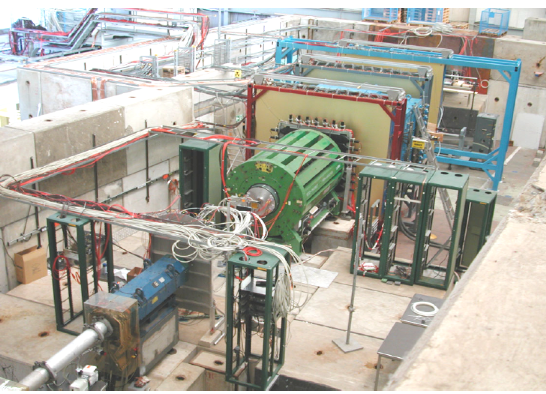
\includegraphics[width=0.8\textwidth]{img/Harp.png}
\caption{\small The HARP experiment at CERN (circa the year 2000). The green cylinder in the center of the setup is the TPC90 magnet } \label{fig.Harp}
\end{figure}

Figure \ref{fig.Harp} shows the experimental area where the HARP neutrino hadro production  experiment took data in the early 2000 (the PI of this proposal was the physics convener of the experiment). The green cylinder is the TPC90 magnet, which produced a very uniform solenoidal field over a region of diameter 1 m and length 3 m. The magnet can operate up to voltages of 0.7 Tesla (we expect that the best performance for NEXT will be around 0.5 T). 

The TPC90 magnet is still available at CERN for the use of recognised experiments, such as NEXT, and currently free. We have already submitted a preliminary request for one year operation (assuming this project is approved). The magnet is an expensive piece of hardware, available from CERN at no cost. The laboratory, will also provide support for the operation of the magnet, as well as a suitable experimental area for the measurements. 

\section*{Objectives of this proposal}
This proposal has two main objectives: 
\begin{enumerate}
\item Upgrade the NEXT-DEMO detector, replacing the energy plane, made of PMTs with a new energy plane made of large area (6$\times$6 mm$^2$) low-noise, ultra-radiopure C-series SENSL SiPMs. A total of 5 boards (4 to be deployed and one spare), hosting 500 SiPMs will be fabricated. In addition, the existing SiPM tracking plane (deploying 1 mm$^2$~Hamamatsu SiPMs mounted in ``old'' cuflon boards) will be replaced with a new tracking plane made with the new kapton dice boards (KDBs) currently in production for NEXT-100. 
\item Operate the upgraded DEMO detector inside the TPC90 solenoid magnet at CERN, in order to study the performance of the system in a magnetic field. A systematic study will be carried on, involving operation at several pressures (between 5 and 15 bar) and magnetic fields (between 0.1 and 0.7 Tesla). 
\end{enumerate}

The goal of this proposal is to: a) demonstrate that good performance (in particular good energy resolution) is obtained by a system based solely in SiPMs operating inside a magnetic field and b) demonstrate that the additional separation between signal and background provided by the magnetic field allows the NEXT experiment to suppress backgrounds by an additional order of magnitude, {\bf therefore becoming the detector with the lowest background rate in the field.} 


\section*{Metodology}
The upgrade of the energy plane requires a new design for the energy KDBs and the corresponding front-end electronics. Such a design, however, is simpler than the existing one for the tracking plane, due to the fact that in the tracking KDBs the signal of each independent pixel must be extracted and amplified, while in the energy KDBs, one can add analogically all the signals in the board (since the gain spread is very small and the energy measurement is an integral). The design, production, testing and certification of the KDBs will be the responsibility of Javier Rodriguez (the electronics engineer in charge of the NEXT tracking plane and the designer of the NEXT KDBs), with the help of technical engineer Vicente Álvarez. 

The energy plane requires purchasing 500 6$\times$6 mm$^2$ low-noise, ultra-radiopure C-series SENSL SiPMs. The sensors will be tested and validated in a setup already available at IFIC for testing the tracking plane SiPMs. After validation they will be mounted in the KDBs, and the whole system will be tested before installation inside DEMO. The new tracking plane requires 4 KDBs and 256 1$\times$1 mm$^2$, all of which are available from NEXT. This part of the project will be carried out by Rodríguez and Álvarez, with the help of one of our graduate students for the SiPM testing. 

After installing the new energy and tracking plane, DEMO will be operated at IFIC, in order to fully characterise the new configuration in the absence of magnetic field. This part of the project will be coordinated by Francesc Monrabal, whose Ph.D. (to be defended in November) has focused in the construction and operation of the NEXT-DEMO between 2011 and 2014. The detector will be calibrated with krypton, caesium, sodium and thorium sources, and the energy resolution as well as the reconstruction of electron tracks will be measured at different pressures and operating conditions. 

Once the detector has been successfully characterised at IFIC, the DEMO setup will be transported to CERN and installed in a suitable experimental area (probably Omega, in the west area of the laboratory). DEMO will be placed inside the TPC90 magnet and the campaign of measurement with radioactive sources will be repeated at different magnetic fields (starting with $B=0$, to reproduce some key results previously obtained at IFIC). The physicist in charge of operations at CERN will be Dr. A. Laing, an experienced post-doc who has served as run coordinator during the DEMO phase. The campaign at CERN will involve a group of 6 physicists, including the PI, Monrabal, Laing and three more post-docs: Dr. Renner, who is leading the magnetic field studies (Kalman filter fit characterisation of signal and background), Dr. Ferrario, who is developing the tracking reconstruction algorithms and  
J. Martin-Albo, who will defend his Ph.D. in December 2014 and has developed the simulation of the detector. The typical operation mode will imply the rotation at CERN of the team members, during a period of four months at CERN.   

\begin{table}[h!]
\begin{center}
\begin{tabular}{| l | c | c | c | c |}
\hline
Tasks & Q1 & Q2 & Q3 & Q4  \\
\hline
Campaign at IFIC & & & &   \\
\hline
Design of the energy plane KDB & m1-m2 & & &   \\
Purchase and testing of SiPMs  & m3 & & &  \\
Mounting and testing of energy plane & & & &  \\
and tracking plane KDBs & & m1  & &  \\
Installing energy plane & & & &  \\
and tracking plane in DEMO & & m2 & & \\
Measurement campaign  & & & & \\
without magnetic field & & m3 & m1 & \\
\hline
Campaign at CERN & & & &   \\
\hline
Transport and installation at CERN & & & m2 &  \\
Commissioning of DEMO and magnet & & & m3 & \\
Measurement campaign & & & & m1-m3 \\
\hline
\end{tabular}
\caption{Timetable for the project. The schedule considers a fast schedule of one year.
Q1-Q4 denote first to fourth quarter. m1-m3 denotes month one to three of each quarter.}
\label{tab:schedule}
\end{center}
\end{table}

Table \ref{tab:schedule} shows the project schedule. The schedule includes contingency and should therefore be met comfortably by the group. The campaign at IFIC takes seven months. One month is foreseen for transport of DEMO to CERN. The campaign at CERN takes four months, one for commissioning and three for measurements. 

From the point of view of personnel, the schedule at CERN will be as follows: Three team members (Monrabal, Laing and the PI) will be present the first month, to ensure a smooth commissioning. During months 2, 3 and 4 (data taking), there will be always 2 team members at CERN in rotating (overlapping) teams. 

\section*{Budget}
Budget is requested for: a) purchase of the energy-plane SiPMs; b) developing and producing the KDBs and front-end electronics for the energy plane; c) transporting DEMO to CERN; d) operation expenses of DEMO at CERN; e) travel and subsistence of the team member while at CERN. 
\begin{table}[!h]
 \begin{center}
    \begin{tabular}{|c|l|cccc|c|}
      \hline
      & Concept & Cost/unit & Units & Subtotal &  Total (VAT included)\\
      \hline
      \multirow{4}{*}{Energy Plane} & SiPMs & 23 & 500 & 11500 & 13915\\
      & Boards & 300 & 10 & 3000  & 3630\\
      & Feedthroughs & 1000 & 1 & 1000  & 1210\\
      & Cables (FT to FE) & 130 & 8 & 1040  & 1258\\
      \hline
      \multirow{7}{*}{Electronics} & SiPM FE: electronics & 968 & 10 &
      9680  & 11713\\
      & SiPM FE: PCB manufacturing & 80.34 & 10 & 803.40  & 972\\
      & SiPM FE: mounting & 114.36 & 10 & 1143.60 &  1384\\
      & Cables (FE to DAQ) & 11.01 & 10 & 110.10 &  133\\
      & FE power supply (HMP4040) & 2334 & 1 & 2334 &
      2824\\
      & 19$^{\prime\prime}$ crates + fan cooling units & 468.27 & 1 & 468.27  & 567\\
      & 100 ft power cable AWG14 & 129.47 & 1 & 129.47  & 157\\
      \hline
      & Total cost & & & & 37363 \\
      \hline
    \end{tabular}
    \caption{Summary of costs of the energy plane: all values in \euro.}
    \label{tab:UpCost}
  \end{center}
\end{table}

Table \ref{tab:UpCost} shows the costs associated with the construction of the new DEMO energy plane.

The cost of the campaign at CERN is as follows: 
\begin{enumerate}
\item We estimate the costs of transport and installation at CERN in 5.000 euros.
\item We estimate the average air fair ticket, flying low-cost in 400 \euro\ per trip. 
\item We estimate one month of hotel at CERN Foyer in 1.500 \euro\ a month (50 \euro\ a day).
\item We limit subsistence expense to 50 \euro\ a day, or 1.500 \euro\ a month.
\item For month 1 (commissioning) we budget 3 trips (1.200 \euro) and 4 weeks of hotel and subsistence for 3 team members (9.000 \euro). 
\item For months 2 to 4 we budget one trip per team member (2.400 \euro) and a total of 20 weeks of hotel and subsistence for the whole team (this includes overlaps between incoming and outgoing shifters), or 15.000 \euro.
\item Therefore, the total cost of the campaign is 32.600 \euro.
\end{enumerate}

The total budget requested is, therefore, 70,000 \euro. 

